\documentclass[12pt]{article}
\usepackage{hyperref}
\usepackage[pdftex]{graphicx}
\usepackage{multirow}
\usepackage{setspace}
\usepackage{color}
\usepackage{multicol}
\usepackage{framed}
\usepackage{mdframed}
\usepackage{lipsum} 
\usepackage{lipsum}

% all 4 borders
\newmdenv{allfour}

\hypersetup{
    bookmarks=true,         % show bookmarks bar?
    unicode=false,          % non-Latin characters in Acrobat’s bookmarks
    pdftoolbar=true,        % show Acrobat’s toolbar?
    pdfmenubar=true,        % show Acrobat’s menu?
    pdffitwindow=false,     % window fit to page when opened
    pdfstartview={FitH},    % fits the width of the page to the window
    pdftitle={My title},    % title
    pdfauthor={Author},     % author
    pdfsubject={Subject},   % subject of the document
    pdfcreator={Creator},   % creator of the document
    pdfproducer={Producer}, % producer of the document
    pdfkeywords={keyword1, key2, key3}, % list of keywords
    pdfnewwindow=true,      % links in new PDF window
    colorlinks=true,       % false: boxed links; true: colored links
    linkcolor=red,          % color of internal links (change box color with linkbordercolor)
    citecolor=green,        % color of links to bibliography
    filecolor=magenta,      % color of file links
    urlcolor=blue           % color of external links
}

\mdfsetup{
  linewidth=.5bp,
  innerleftmargin=3.5bp,
  innerrightmargin=3.5bp,
  innertopmargin=.5bp,
  innerbottommargin=.5bp,
}

% Tristan Hill
% ME4140 - Fall 2016 - Fall 2017

\textwidth=6.5in
\topmargin=-0.5in
\textheight=9.25in
\hoffset=-0.5in
\footskip=0.2in

\pagestyle{myheadings}
\markright{{\large ME 4140 Fall 2018---The Robotic Operating System}}

%\definecolor{mygray}{rgb}{.6, .6, .6}
%\definecolor{mypurple}{rgb}{0.6,0.1961,0.8}
\definecolor{mygreen}{rgb}{0.1333 ,  0.5451,    0.1333}
\definecolor{mypink}{rgb}{0.1333 ,  0.5451,    0.1333}


\definecolor{mygreen}{rgb}{0, .39, 0}

%\definecolor{dred}{#8B0000}
% [153,50,204] - dark orchid
\definecolor{mypurple}{rgb}{0.6,0.1961,0.8}
%[139,69,19] - saddle brown
\definecolor{mybrown}{rgb}{0.5451,0.2706,0.0745}
\definecolor{mygray}{rgb}{.6, .6, .6}

\definecolor{mygray}{rgb}{.6, .6, .6}

\newcommand{\VA}{\vspace{2mm}}
\newcommand{\VB}{\vspace{5mm}} 
\newcommand{\VC}{\vspace{30mm}} 
 
\newcommand{\R}{\color{red}}
\newcommand{\B}{\color{blue}}
\newcommand{\K}{\color{black}}
\newcommand{\G}{\color{mygreen}}
\newcommand{\PR}{\color{mypurple}}
\newcommand{\GY}{\color{mygray}}

\begin{document}

\thispagestyle{plain}

\begin{center}
	   {\bf \Large Installing the {\underline{\LARGE Ubuntu Linux}} Operating System}\vspace{5mm} \\
   {\bf \large ME 4140 - Introduction to Robotics - Fall 2017} \vspace{5mm}\\
\end{center}

\large
\begin{enumerate}

		\item If your Ubuntu Operating System is running you are ready to install ROS! 
		\href{http://wiki.ros.org/kinetic/Installation/Ubuntu}{Website} \\\\
		\item Open a terminal and enter the commands in the red boxes in order.\\\\
				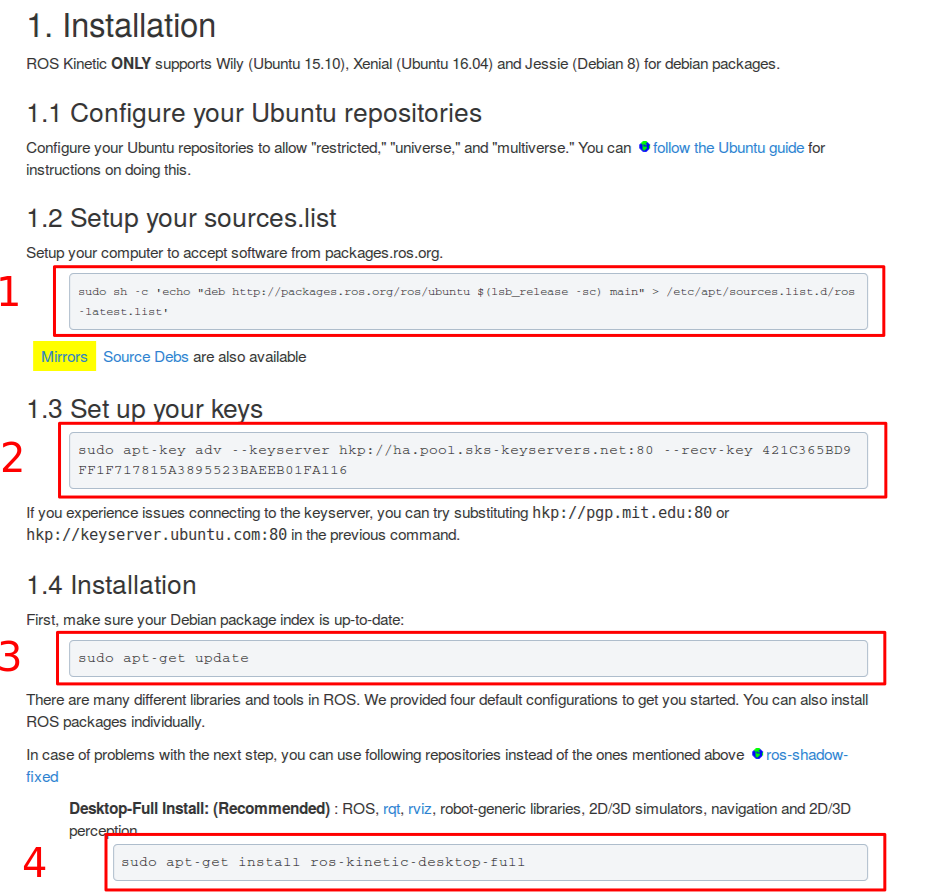
\includegraphics[scale=.5]{os_install_fig14.png}\\
		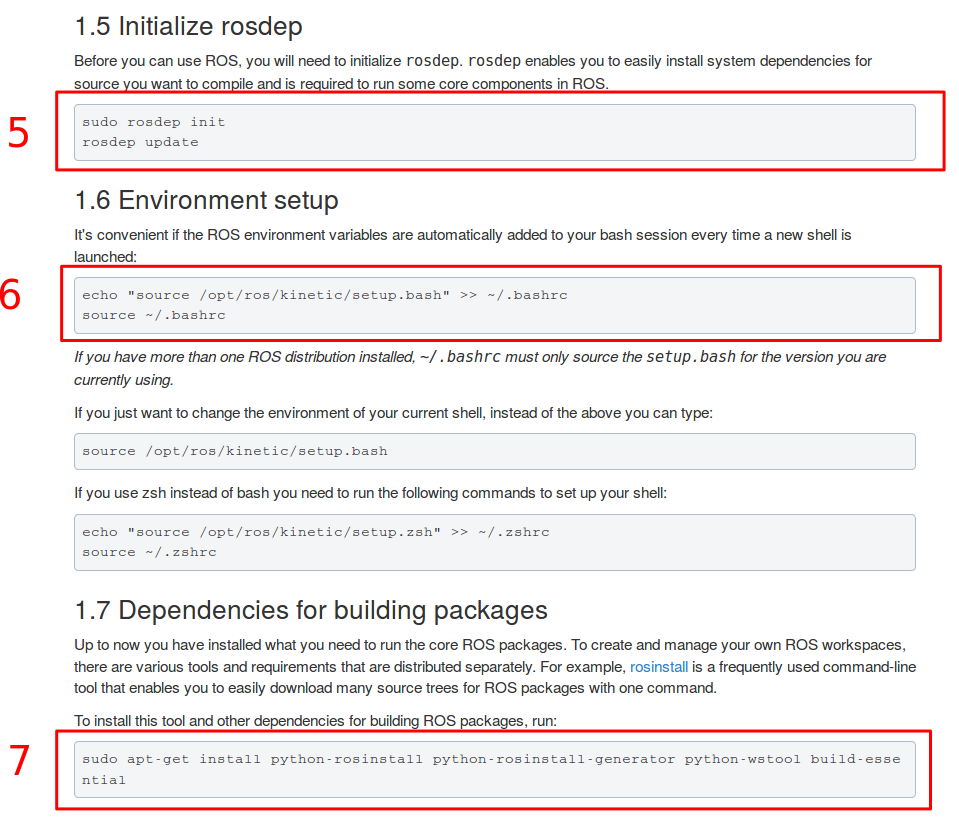
\includegraphics[scale=.5]{os_install_fig15.png}\\

		\item Close the terminal. Open a new terminal and try the following command:
		
			\$ roscore

\end{enumerate}

\end{document}
\